\documentclass[nobib]{tufte-handout}

\title{Lecture 4: Spectral graph theory and the matrix-tree theorem $\cdot$ 1MA020}

\author[Vilhelm Agdur]{Vilhelm Agdur\thanks{\href{mailto:vilhelm.agdur@math.uu.se}{\nolinkurl{vilhelm.agdur@math.uu.se}}}}

\date{3 November 2023}


%\geometry{showframe} % display margins for debugging page layout

\usepackage{graphicx} % allow embedded images
  \setkeys{Gin}{width=\linewidth,totalheight=\textheight,keepaspectratio}
  \graphicspath{{graphics/}} % set of paths to search for images
\usepackage{amsmath}  % extended mathematics
\usepackage{booktabs} % book-quality tables
\usepackage{units}    % non-stacked fractions and better unit spacing
\usepackage{multicol} % multiple column layout facilities
\usepackage{lipsum}   % filler text
\usepackage{fancyvrb} % extended verbatim environments
  \fvset{fontsize=\normalsize}% default font size for fancy-verbatim environments

\usepackage{color,soul} % Highlights for text

% Standardize command font styles and environments
\newcommand{\doccmd}[1]{\texttt{\textbackslash#1}}% command name -- adds backslash automatically
\newcommand{\docopt}[1]{\ensuremath{\langle}\textrm{\textit{#1}}\ensuremath{\rangle}}% optional command argument
\newcommand{\docarg}[1]{\textrm{\textit{#1}}}% (required) command argument
\newcommand{\docenv}[1]{\textsf{#1}}% environment name
\newcommand{\docpkg}[1]{\texttt{#1}}% package name
\newcommand{\doccls}[1]{\texttt{#1}}% document class name
\newcommand{\docclsopt}[1]{\texttt{#1}}% document class option name
\newenvironment{docspec}{\begin{quote}\noindent}{\end{quote}}% command specification environment

\include{mathcommands.extratex}

\begin{document}

\maketitle% this prints the handout title, author, and date

\begin{abstract}
\noindent
We introduce the basic notions of spectral graph theory, such as the adjacency and incidence matrices of a graph. We build up the theory around these, eventually arriving at the Kirchhoff matrix-tree theorem, which will let us count spanning trees in a graph.
\end{abstract}

Throughout this lecture, we will assume that $G = (V, E)$ is a graph on $n$ vertices, with vertex set $[n]$, and $m$ edges $\{e_1, \ldots, e_m\}$.

\section{Adjacency matrices}

\begin{definition}
    The \emph{adjacency matrix} $A$ of a graph $G$ is the $n\times n$ matrix having entries $A_{ij} = 1$ if $i$ and $j$ are neighbours, and zero otherwise.
\end{definition}

\begin{figure}
    \centering
    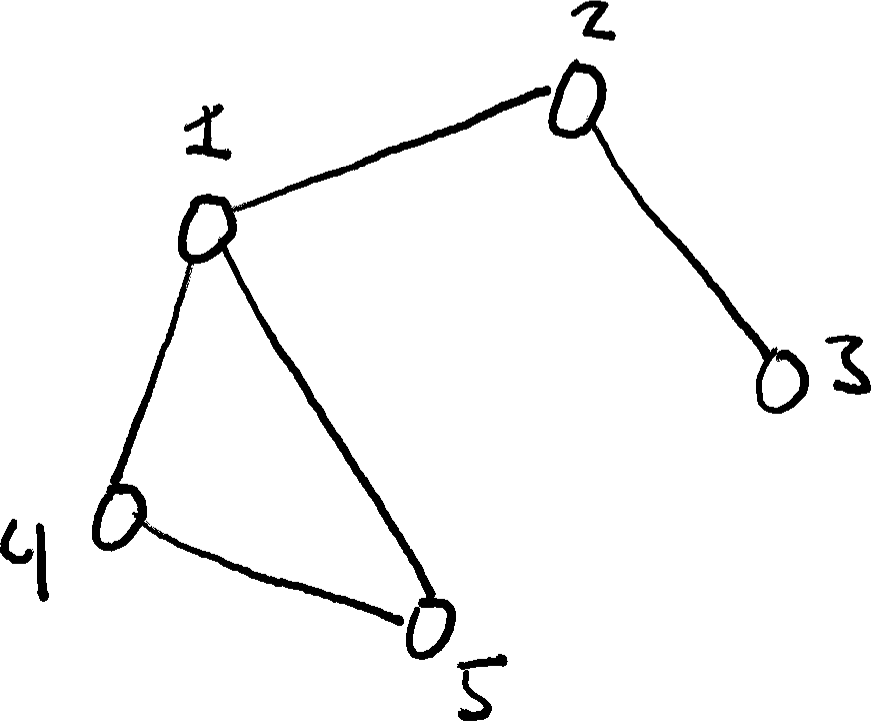
\includegraphics[width=0.3\textwidth]{graphics/L4_spectral/graph_for_adjmat.png}
    \caption{A graph whose adjacency matrix we compute in an example.}
    \label{fig:graph_for_adjmat}
\end{figure}

\begin{example}
    The graph given in Figure \ref{fig:graph_for_adjmat} has adjacency matrix
    $$\begin{pmatrix}
        0 & 1 & 0 & 1 & 0 \\
        1 & 0 & 1 & 0 & 0 \\
        0 & 1 & 0 & 0 & 0 \\
        1 & 0 & 0 & 0 & 1 \\
        0 & 0 & 0 & 1 & 0 
        \end{pmatrix}.$$
\end{example}

\begin{remark}
    There are a few things we can notice immediately about adjacency matrices. First off, they must be symmetric, since of course $i$ and $j$ being neighbours is the same statement as $j$ and $i$ being neighbours, and the diagonal entries are always zero. Second, the row sums or the column sums give us the degree of each vertex, since a row contains one $1$ per edge incident to its vertex.

    Finally, it follows from the spectral theorem for symmetric matrices that all eigenvalues of $A$ are real.
\end{remark}

\section{Incidence matrices}

There is another way to turn a graph into a matrix that is very useful, but it is easiest to define it first for directed graphs, so we begin by giving a definition of a directed graph.

\begin{definition}
    A \emph{directed graph} $G = (V,E)$ (or \emph{digraph} for short) consists of a set of vertices $V$ and a set of edges $E$, where each edge is a tuple of two distinct\sidenote[][]{It is entirely possible to define what we mean by a directed multigraph as well, but for our purposes, we stick to simple directed graphs with no loops or parallel edges.} vertices. We call the first vertex in the tuple the \emph{source} and the second vertex the \emph{target} of the edge.
\end{definition}

Having said this, we can now define the incidence matrix of a directed graph.

\begin{definition}
    The \emph{incidence matrix} $D$ of a digraph $G$ is the $n\times m$ matrix having entries $D_{ij}$, where
    \begin{equation*}
        D_{ij} = \begin{cases}
            1 &\text{if } i \text{ is the target of } e_j\\
            -1 &\text{if } i \text{ is the source of } e_j\\
            0 &\text{otherwise.}
        \end{cases}
    \end{equation*}

    For a simple graph $G$ and a matrix $D$, we say that $D$ is \emph{an} incidence matrix of $G$ if there is a way to direct the edges of $G$ so that the incidence matrix of this directed version is $D$.
\end{definition}

\begin{figure}
    \centering
    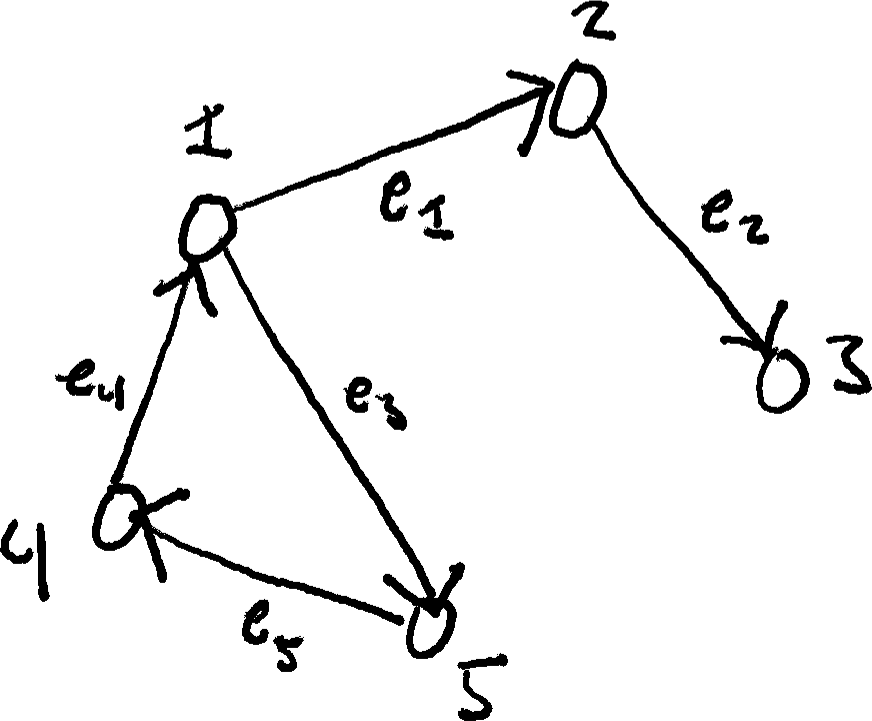
\includegraphics[width=0.5\textwidth]{graphics/L4_spectral/digraph_for_incmat.png}
    \caption{A way of directing the edges of the graph in Figure \ref{fig:graph_for_adjmat}. We have also labelled the edges with their numbers.}
    \label{fig:digraph_for_incmat}
\end{figure}

\begin{example}
    In Figure \ref{fig:digraph_for_incmat} we see one way of directing the edges of the graph in Figure \ref{fig:graph_for_adjmat} to make it a digraph. This digraph has incidence matrix\sidenote[][]{It is a bit unfortunate that our example graph has exactly one cycle, so it has equally many edges and vertices and the incidence matrix is square -- they are of course not in general square.}
    $$\begin{pmatrix}
        -1 & 0 & -1 & 1 & 0 \\
        1 & -1 & 0 & 0 & 0 \\
        0 & 1 & 0 & 0 & 0 \\
        0 & 0 & 0 & -1 & 1 \\
        0 & 0 & 1 & 0 & -1 
        \end{pmatrix}$$
    and so this matrix is also an incidence matrix for our original simple graph.
\end{example}

Having given these definitions, let us start seeing why these matrices are interesting.

\begin{lemma}\label{lemma:ranks_of_incidence_matrix}
    Let $G$ be a finite simple graph on $n$ vertices with $c$ connected components, and $D$ be an incidence matrix of $G$. It holds that
    $$\rank D = n - c.$$

    \begin{proof}
        To begin with, let us see that $\rank D \leq n - 1$. The column sums of $D$ are all zero, since each column contains exactly one $1$ and one $-1$, for the source and target of its associated edge. Therefore, if we take the sum of all the \emph{row}-vectors, each entry will be zero, so we have a non-trivial linear combination of $0$, and hence $\rank D \leq n - 1$.

        Now, assume $G$ is in fact connected -- then, we will show that this linear combination of $0$ is in fact, up to scaling, the only non-trivial linear combination of $0$ with the row-vectors. So, let $r_i$ for $i = 1,\ldots,n$ denote the row-vectors of $D$, and suppose we have a non-trivial linear combination
        $$\sum_{i=1}^n \alpha_i r_i = 0.$$

        Consider a row $k$ for which $\alpha_k \neq 0$ -- in this row, there is a non-zero entry in every column corresponding to an edge incident to the vertex $k$. Each of these columns has one other non-zero entry, and that entry has the opposite sign of the one in our row. So for these to sum to zero, the coefficients in the linear combination must be the same. So what we have seen is that $\alpha_\ell = \alpha_k$ whenever $\ell$ is adjacent to $k$.

        However, we assumed $G$ is connected, so this argument in fact extends to showing that all the coefficients must equal $\alpha_k$, and so this shows the linear combination is indeed just a rescaling of the sum of all the rows.

        Finally, assume $G$ has $c$ connected components, and observe that we can always relabel the vertices and edges in such a way that $D$ is in block-diagonal form, with every block being the incidence matrix of a connected component. So the claim follows from the statement for connected graphs.
    \end{proof}
\end{lemma}

The statement we are looking towards, counting spanning trees, will involve determinants, so let's start proving things about determinants of these matrices.

\begin{lemma}\label{lemma:square_submats_of_incmat}
    Any square submatrix of an incidence matrix $D$ has determinant $0$, $1$, or $-1$.

    \begin{proof}
        We prove this by induction in the size $k$ of the $k\times k$ submatrix. The statement is obvious for $k=1$, since all the entries of an incidence matrix are zero, one, or minus one.

        Now consider a submatrix $M$ of size $(k+1)\times(k+1)$. If every column of $M$ has either two or no non-zero entries, then $\det M = 0$, since then every column will sum to zero. Otherwise, there is a column of $M$ having exactly one non-zero entry. Expanding $m$ along this column yields $\det M = \pm \det M'$ where $M'$ is a $k \times k$ submatrix of $D$. Hence the result follows by induction.
    \end{proof}
\end{lemma}

Now, consider what happens if we pick some set of edges $S \subset E$, and let $D_S$ be just the columns of the incidence matrix that correspond to these edges -- this will in fact be the incidence matrix of the spanning subgraph $(V, S)$ of $G$. So if we pick $S$ as a set of $n-1$ edges, this spanning subgraph will be a spanning tree exactly if it is connected\sidenote[][]{
    \begin{xca}
        Prove that a graph on $n$ vertices and $n-1$ edges is a tree if and only if it is connected.
    \end{xca}
} -- and Lemma \ref{lemma:ranks_of_incidence_matrix} gives us a nice way of checking if it is connected or not: It is connected whenever $\rank D_S = n - 1$.

\begin{lemma}\label{lemma:invertible_iff_spanningtree}
    Let $S$ be an $n-1$-element subset of the edges of $G$, and let $M$ denote any $(n-1)\times (n-1)$ submatrix of the $n \times (n-1)$ matrix $D_S$. Then $M$ is invertible if and only if $(V,S)$ is a spanning tree of $G$.

    \begin{proof}
        We already observed that $D_S$ has rank $n-1$ whenever $(V,S)$ is a spanning tree, so removing any row from it will create a non-singular square matrix $M$.

        In the other direction, if $M$ is nonsingular, then $D_S$ contains at least $n-1$ linearly independent rows and the same number of linearly independent columns. Hence $\rank D_S = n - 1$ and so $(V,S)$ must be connected and thus a tree, since it has $n-1$ edges.
    \end{proof}
\end{lemma}

\section{The Laplacian matrix}

We have now gotten to the point where we can introduce the final matrix associated to a graph that we want to study.

\begin{definition}
    Let $G$ be a finite simple graph. Denote its adjacency matrix by $A$, and let $\Delta$ be a diagonal $n\times n$ matrix having diagonal entries $\Delta_{ii} = d_i$ for each $i$. Then, the \emph{Laplacian matrix} $Q$ of $G$ is given by
    $Q = \Delta - A.$
\end{definition}

The reason we define this matrix is because it connects the adjacency and incidence matrices in a nice way.

\begin{theorem}
    Let $G$ be a finite simple graph, $A$ its adjacency matrix, $D$ an incidence matrix for $G$, and $Q$ its Laplacian matrix. Then it holds that
    $$Q = DD^t = \Delta - A.$$

    Notice that in particular this means that $DD^t$ is the same for every incidence matrix, independent of the orientation chosen of the edges.

    \begin{proof}
        The entry $(DD^t)_{ij}$ is the inner product of rows $r_i$ and $r_j$ of $D$.

        If $i = j$, this amounts to summing the squares of the entries in $r_i$, and there are $d_i$ of them, each $\pm 1$, so the sum of their squares is just $d_i$, as needed.
        
        Now, if $i \neq j$, there is a non-zero entry in position $\ell$ in both $r_i$ and $r_j$ precisely when $e_\ell$ is an edge between $i$ and $j$ -- and this entry has to be $(1)(-1) = -1$. Since we assumed $G$ is simple, there can be at most one edge between $i$ and $j$. So we have seen that $(DD^t)_{ij}$ is $-1$ if $\{i,j\}$ is an edge, and zero otherwise.
    \end{proof}
\end{theorem}

In order to arrive at the result we are looking for, we will need some heavier linear-algebraic machinery.

\begin{definition}
    Suppose $M$ is a square matrix. A \emph{cofactor} $M_{ij}$ of this matrix is the determinant of the submatrix of $M$ in which row $i$ and column $j$ have been removed.

    If we consider the matrix whose entries are the cofactors, and take its transpose, we get the \emph{adjugate matrix} of $M$, denoted $\adj M$.
\end{definition}

Let us gather some linear-algebraic facts we will need and use without proof in one lemma:

\begin{lemma}\label{lemma:linear_algebra_facts}
    Let $M$ be an arbitrary $n\times n$ matrix. It holds that
    \begin{enumerate}
        \item $M(\adj M) = (\det M)I_n$.
        \item If $M$ is symmetric, so is $\adj M$.\sidenote[][]{This one is perhaps nearly obvious, but still good to state explicitly.}
        \item Suppose $M$ is symmetric and the row- and column-sums of $M$ are all zero, and let the non-zero eigenvalues of $M$ be $\lambda_1, \ldots, \lambda_{n-1}$. Then any cofactor of $M$ is equal to $\frac{1}{n}\lambda_1\ldots\lambda_n$.
    \end{enumerate}
\end{lemma}

\begin{lemma}
    Let $Q$ be the Laplacian matrix of a graph $G$, and denote by $J$ the $n\times n$ matrix all of whose entries are $1$. Then $\adj Q$ is a scalar multiple of $J$.

    \begin{proof}
        We observe first that $\rank Q = \rank D$. So if $G$ is disconnected, then we know by Lemma \ref{lemma:ranks_of_incidence_matrix} that $\rank Q < n - 1$, so all the $(n-1)\times(n-1)$ matrices determining the cofactors must also be singular, and thus $\adj Q = 0$.

        Now, if $G$ is connected, we get that $\rank Q = n - 1$ and thus $\det Q = 0$, and so 
        $$Q(\adj Q) = (\det Q)I_n = 0.$$

        That $Q(\adj Q) = 0$ implies that every column vector of $\adj Q$ is in the kernel of $Q$. Now, since $\rank Q = n - 1$, this kernel is one-dimensional -- in fact, it is spanned by $(1,1,\ldots,1)^t$, since we can compute
        \begin{align*}
            Q_{i, \cdot}\cdot(1,1,\ldots,1)^t &= (\Delta - A)_{i, \cdot}(1,1,\ldots,1)^t\\
            &= d_i - \sum_{j \sim i} 1 = 0.
        \end{align*}

        So it follows that every column of $\adj Q$ is a scalar multiple of $(1,1,\ldots,1)^t$ -- but since $Q$ is symmetric, so is $\adj Q$, and thus all these scalar multiples have to be the same, proving the lemma.
    \end{proof}
\end{lemma}

So we have shown that all these cofactors are in fact equal -- so the final step is to show that they are actually the number of spanning trees of the graph. To see this, we need one final big hammer from linear algebra.

\begin{theorem}[Cauchy-Binet]
    Let $A$ and $B$ be two $n\times m$ matrices, with $n \leq m$. For any set $S\subseteq [m]$, denote by $A_S$ ($B_S$) the submatrix of $A$ ($B$) acquired by picking only the columns in $S$. Then
    $$\det\left(AB^t\right) = \sum_{\substack{S \subseteq [m]\\\abs{S} = n}} \det\left(A_S\right)\det\left(B_S\right).$$
\end{theorem}

Now we can finally state and prove the Kirchhoff matrix-tree theorem:

\begin{theorem}[Kirchhoff's matrix-tree theorem]
    Let $G$ be a finite simple graph with Laplacian $Q$. Then any cofactor of $Q$ equals $t(G)$, the number of spanning trees of $G$,\sidenote[][]{Note that this is the part of the theorem that gives a good algorithm for computing the number of spanning trees: The Laplacian is trivial to compute, and computing a cofactor of it just requires you to compute a single determinant. The second half of the statement, on the other hand, would require you to compute the entire spectrum of the graph, which is notably more computation.} and if $\lambda_1, \lambda_2, \ldots, \lambda_{n-1}$ are the non-zero eigenvalues of $Q$, then
    $$t(G) = \frac{1}{n}\prod_{i=1}^{n-1}\lambda_i.$$

    \begin{proof}
        We've already proven that all the cofactors are equal, so we can focus on just a single cofactor. Let $D$ be an incidence matrix of $G$, and let $\Tilde{D}$ be $D$ with its last row removed. Then $\det\left(\Tilde{D}\Tilde{D}^t\right)$ is a cofactor of $Q = DD^t$, and we can express this cofactor using the Cauchy-Binet theorem as
        $$\det\left(\Tilde{D}\Tilde{D}^t\right) = \sum_{\substack{S \subseteq E\\\abs{S} = n - 1}} \left(\det \Tilde{D}_S\right)^2.$$

        Now, we know from Lemma \ref{lemma:square_submats_of_incmat} that the determinant of a square submatrix of an incidence matrix always has determinant $-1$, $1$, or $0$,\sidenote[][]{So since $\Tilde{D}$ is a submatrix of $D$, a square submatrix of $\Tilde{D}$ is a square submatrix of $D$ as well.} so each summand on the right is either $0$ or $1$. However, we know from Lemma \ref{lemma:invertible_iff_spanningtree} that such a square matrix is invertible -- and thus has non-zero determinant -- if and only if the corresponding spanning subgraph is a spanning tree. So the right hand sum in fact counts spanning trees.

        That the second statement of the theorem follows from the first is exactly the third statement of Lemma \ref{lemma:linear_algebra_facts}.
    \end{proof}
\end{theorem}

Having arrived at our big result, let us now -- as promised -- use it to give a proof of Cayley's formula.

\begin{proof}[Proof of Cayley's formula]
    The key observation here is that a tree whose vertices are labelled from $1$ through $n$ is precisely a spanning tree of the complete graph on $n$ vertices, if we label also its vertices by $1$ through $n$. So if we apply the matrix-tree theorem to the complete graph, we will get a count of the labelled trees on $n$ vertices.

    It is easy to see that the Laplacian of $K_n$ is
    $$\begin{pmatrix}
        n-1 & -1 & \dots & -1 \\
        -1 & n-1 & \ddots & \vdots \\
        \vdots & \ddots & \ddots & -1 \\
        -1 & \dots & -1 & n-1
       \end{pmatrix}$$
    and as expected the vector $(1,1,\ldots,1)^t$ is an eigenvector for the eigenvalue $0$. A little bit of thought reveals that there are $n-1$ other eigenvectors of the form $(0,\ldots,0,1,-1,0,\ldots,0)^t$ all corresponding to the eigenvalue $n$. Hence
    $$t(K_n) = \frac{1}{n}n^{n-1} = n^{n-2}$$
    as desired.
\end{proof}

\section{Exercises}

\begin{xca}
    The definition of the adjacency matrix extends in a natural way to directed graphs -- we say that $A_{ij}$ is $1$ whenever there is an edge from $i$ to $j$. So this matrix is no longer necessarily symmetric.

    It is of course never possible for a matrix to have the same adjacency matrix and incidence matrix, because the former has no negative entries while the latter, if it has any entries, has at least one negative entry. However, it is not as immediately obvious whether it is possible for $A - A^t = D$ to happen for a directed graph $G$.\sidenote[][]{If this did happen, one might call this adjacency-and-incidence matrix a \emph{coincidence matrix}.}\sidenote[][]{Yes, I gave this exercise entirely because of the pun.}

    Is this in fact possible? If so, for which graphs does it happen?
\end{xca}

%\bibliography{references}
%\bibliographystyle{plainnat}

\end{document}
